\section{MOA \& Privacy Filters}
\label{Implementation:PrivacyFilter}

\textbf{Notation:} from now on, a text stylized with a monospaced font like \texttt{this example} will refer to an actual programming artifact: a variable, class, file name, etc.

We have already showed along this report that \textit{filters} are a feature of the MOA framework. Filters are, actually, a particular form of \textit{stream}. Whenever a filter should be applied to a stream to perform a posterior analysis, a \texttt{FilteredStream}\footnote{All documentation of the MOA API can be found on \url{http://www.cs.waikato.ac.nz/~abifet/MOA/API/index.html}} is built. This class takes a generic \texttt{Stream} object as the input stream and a list of \texttt{StreamFilter}s, which are also \texttt{Stream}s, if we examine their type hierarchy. Taking advantage of the existence of both the \texttt{FilteredStream} and \texttt{StreamFilter} classes, we can begin designing the privacy filters that will implement the actual SDC methods.

\subsection{\texttt{PrivacyFilter}}
\label{Implementation:PrivacyFilter:PrivacyFilter}

Thanks to the object-oriented capabilities of the Java language, we can design and implement a generic abstract data type for all proposed SDC algorithms. By doing so, we will be able to centralize some of the common logic behind them. The abstract type of the privacy filters is the \texttt{PrivacyFilter} class. An incomplete UML diagram of the specification of this class and its most relevant parent types can be seen in~\fref{fig:privacy-filter-uml}.

Concerning the responsibility\footnote{In object-oriented programming, the \textit{single responsibility principle} states that every class should have responsibility over a single part of the functionality provided by the software, and that responsibility should be entirely encapsulated by the class (\citet{web:SOLID}).} of this class, there is a main task that the \texttt{PrivacyFilter} is meant to address: the measurement or \textit{evaluation} of the \textbf{disclosure risk} (DR) and the \textbf{information loss} (IL). The approach is to let the SDC method (the \textit{concrete} subclass) anonymize the \textit{instances}\footnote{In the MOA context, records in a dataset (in a stream) are called \textit{instances} and are represented using the \texttt{Instance} interface.} of the stream and collect them, along with the original instances that have been processed. The evaluation of both magnitudes, DR and IL, is performed using these \textit{pairs} of instances. The mechanism is best understood with the schematic presented in~\fref{fig:privacy-filter-schematic}.

\begin{figure}[h]
	\centering
	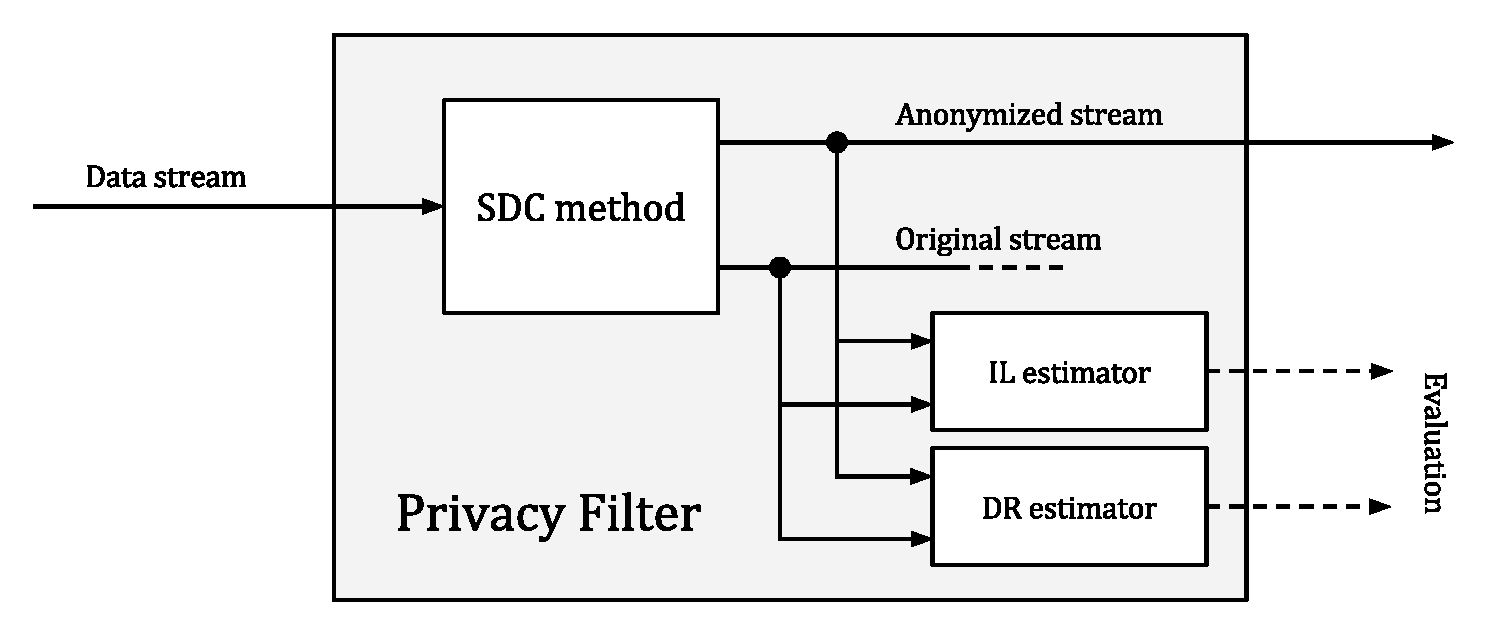
\includegraphics[width=0.8\textwidth]{figures/privacy-filter-schematic.pdf}
	\caption{A schematic of the tasks performed by the \texttt{PrivacyFilter} class, showing the stream data flow.}
	\label{fig:privacy-filter-schematic}
\end{figure}

\subsubsection*{Implementation details}
\label{Implementation:PrivacyFilter:PrivacyFilter:Details}

The \texttt{PrivacyFilter} class is, by construction, an \texttt{InstanceStream} and a \texttt{StreamFilter} (see~\fref{fig:privacy-filter-uml}) but also, and most importantly, an \texttt{AnonymizationFilter}. This last \textit{interface}, which the \texttt{PrivacyFilter} implements, allows to encapsulate all privacy-preserving behaviour in a single module.

The most important of the methods defined in the \texttt{AnonymizationFilter} type is

\begin{center}
	\texttt{nextAnonymizedInstancePair() : InstancePair}
\end{center}

which is left to be implemented (it is \textit{abstract} at the \texttt{PrivacyFilter} level) by any subclass. This way, we can use \textit{inversion of control}\footnote{The \textit{Hollywood principle} or \textit{inversion of control} pattern is a software design methodology that takes its name from the cliché response given to amateurs auditioning in Hollywood: "Don't call us, we'll call you". It is a useful paradigm that assists in the development of code with high cohesion and low coupling that is easier to debug, maintain and test.} to force a subtype define the concrete behaviour of the function, while still conforming to a precise \textit{contract}. The \texttt{InstancePair} returned by this abstract method is just a tuple containing both the original and anonymized instances that should be streamed next.

\begin{figure}[h]
	\centering
	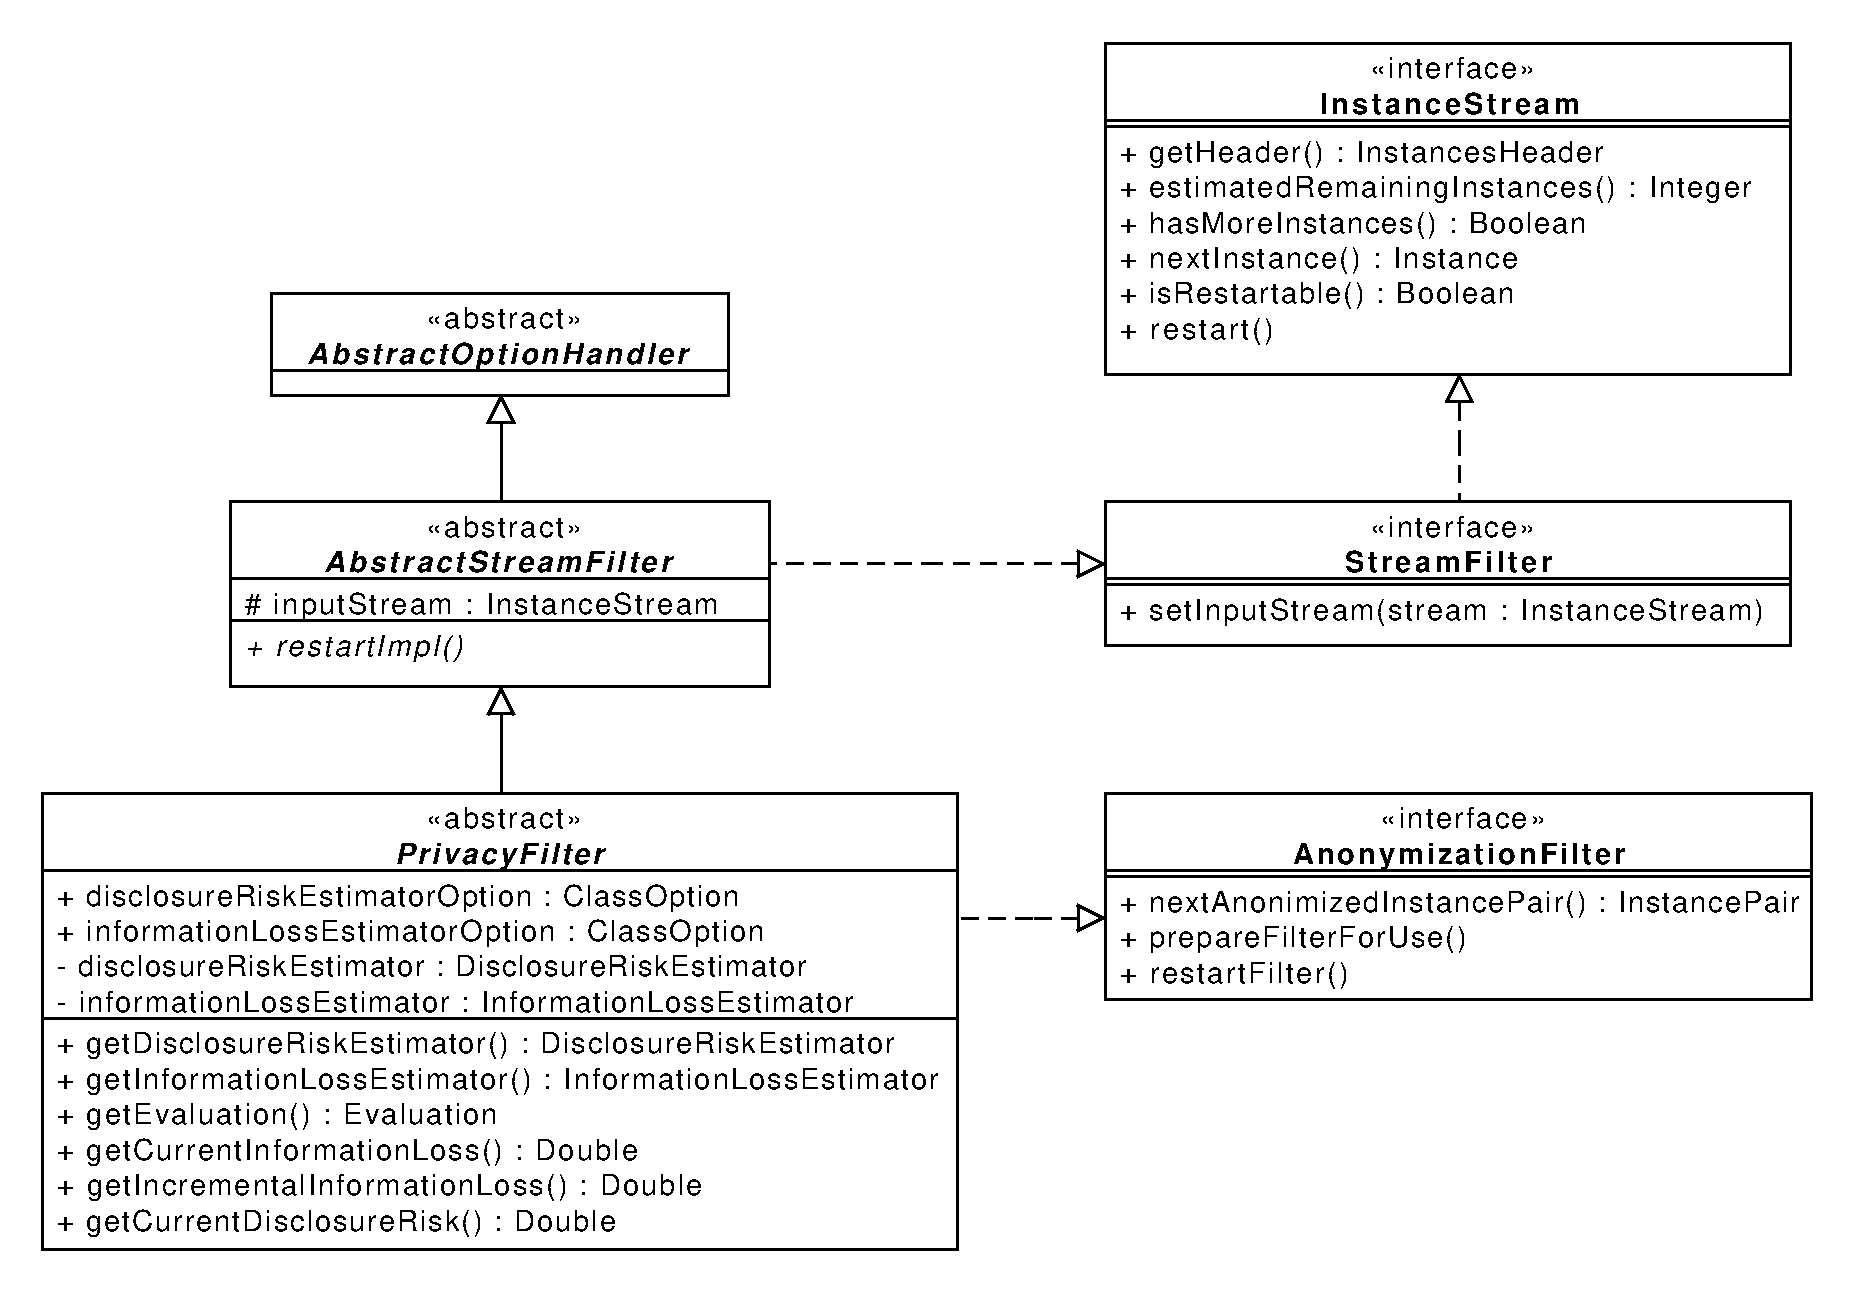
\includegraphics[width=1.0\textwidth]{figures/class_PrivacyFilter.pdf}
	\caption{UML class diagram of the relevant types in the \texttt{PrivacyFilter} class hierarchy. Notice that not all the involved types are shown.}
	\label{fig:privacy-filter-uml}
\end{figure}

\subsubsection*{Estimators}
\label{Implementation:PrivacyFilter:PrivacyFilter:Estimators}

The estimators used by the \texttt{PrivacyFilter} class are desgined to be modular and, most of all, easily modifiable: they are just interfaces defining a simple contract that all estimators must implement. The methods belonging to such contracts can be seen in~\fref{fig:estimators-uml} (the concrete estimators implementation is explained in~\sref{Implementation:Estimators}).

\begin{figure}[h]
	\centering
	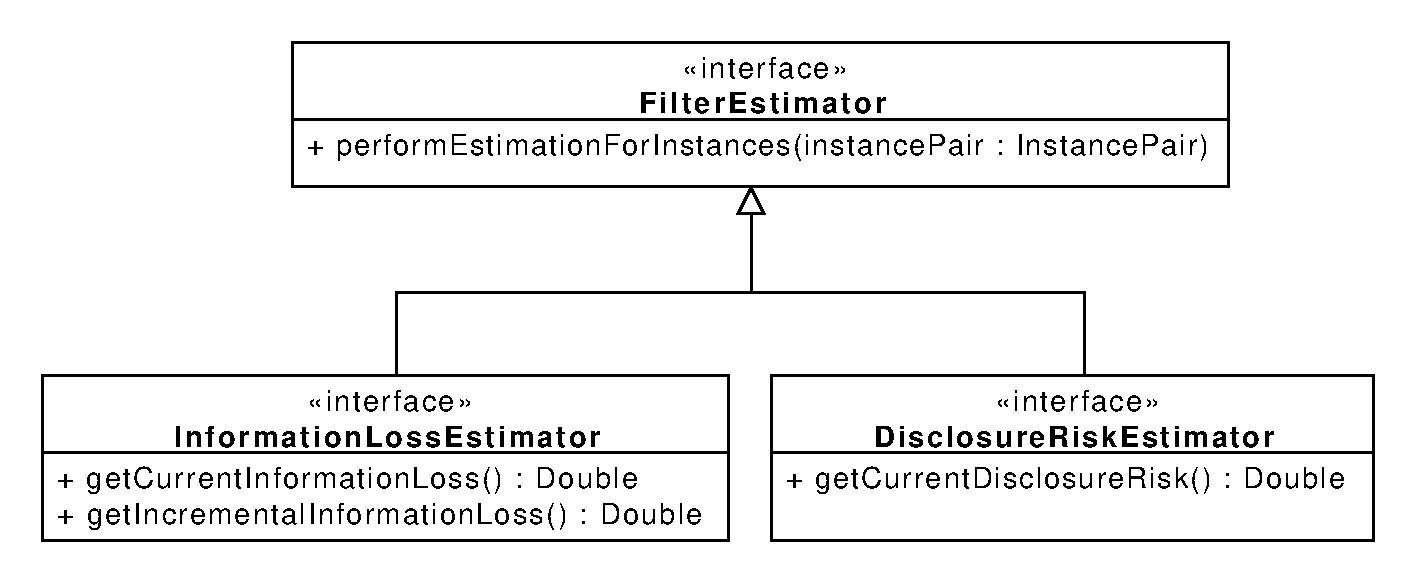
\includegraphics[width=0.8\textwidth]{figures/class_Estimators.pdf}
	\caption{Class diagram of the \texttt{FilterEstimator} type hierarchy.}
	\label{fig:estimators-uml}
\end{figure}

Finally, the disclosure risk and information loss estimators used by a \texttt{PrivacyFilter} can be configured at runtime by setting the appropriate \textit{options}\footnote{The MOA framework makes extensive use of configurable \textit{options}, which can be set either on a command line execution or via the GUI that MOA provides.} of the filter (see~\sref{Implementation:Deployment:Examples} for examples on how to use the MOA framework and the privacy filters extension).

\subsection{Filters ecosystem}
\label{Implementation:PrivacyFilter:Ecosystem}

Having reviewed the basic \texttt{PrivacyFilter} generic type, we can now provide a couple of figures that introduce the final structure of the privacy filters class ecosystem. The \textit{package} encapsulation of the methods can be seen on~\fref{fig:moa-ppsm-packages}. An incomplete\footnote{Most of the classes shown in the diagram depend on others for their internal implementation, but, for the sake of concreteness, they are not shown, as are not relevant for the purpose of this report.} class diagram of the filters is shown in~\fref{fig:moa-ppsm-class-uml}.

\begin{figure}
	\centering
	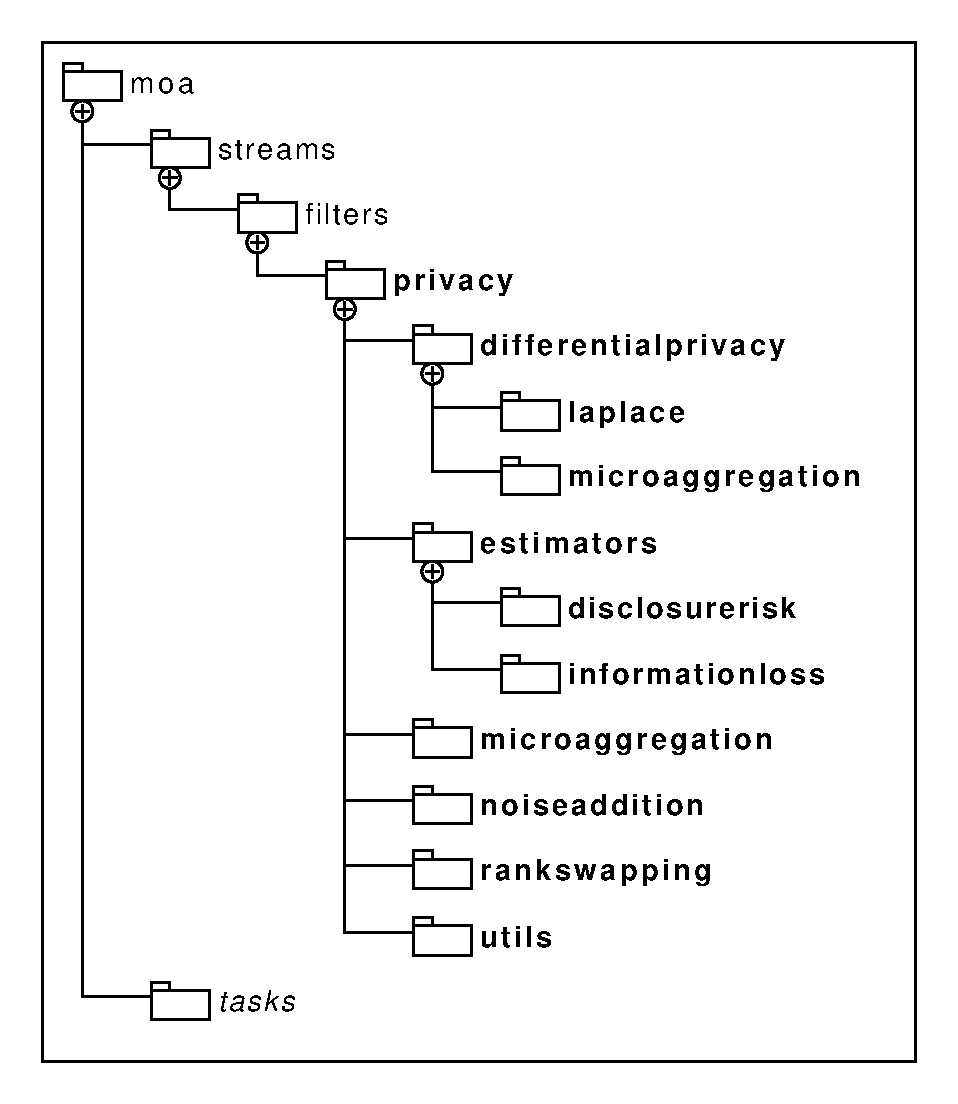
\includegraphics[width=0.5\textwidth]{figures/moa-ppsm-packages.pdf}
	\caption{Package organization of the privacy filters. \textbf{New} packages (not existing in the MOA framework) are shown in bold. \textit{Existing} packages that have been extended with new types are shown in italics.}
	\label{fig:moa-ppsm-packages}
\end{figure}

\begin{figure}
	\centering
	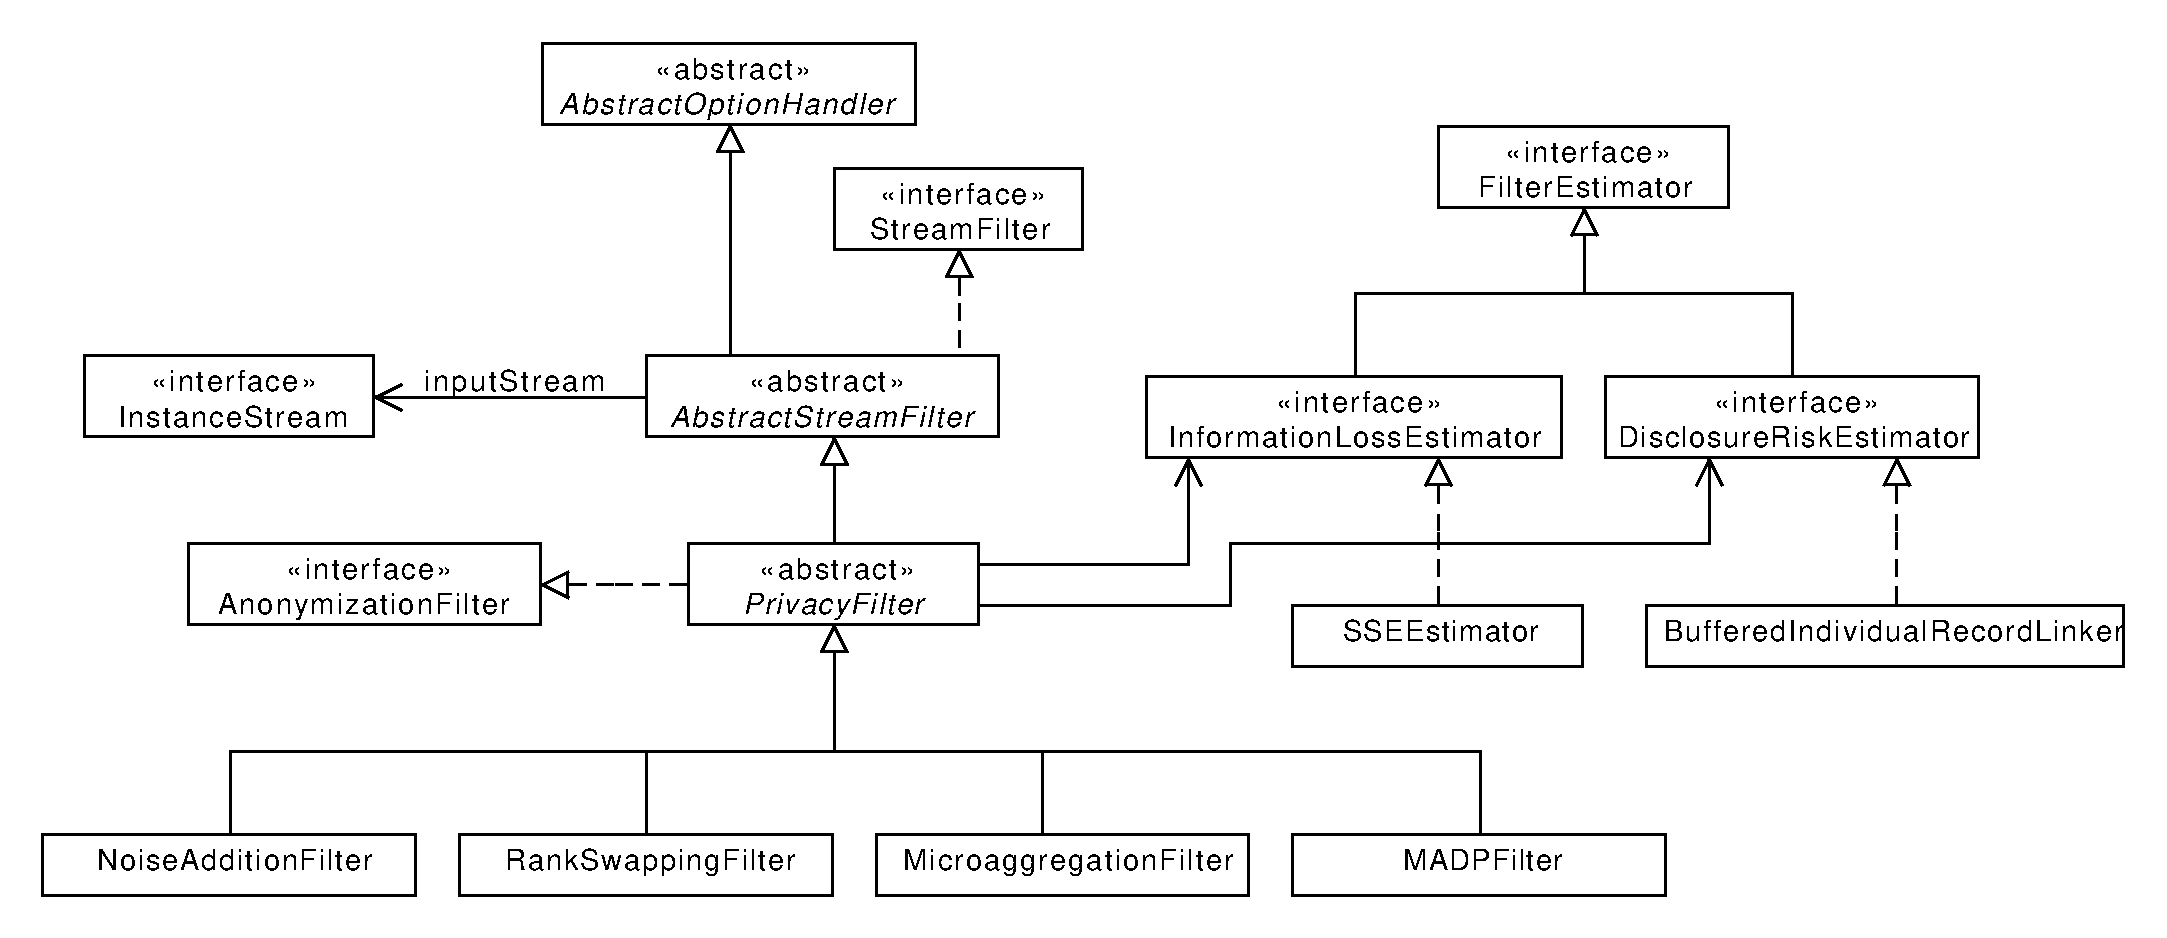
\includegraphics[width=1.0\textwidth]{figures/refactored-ppsm-class-diagram.pdf}
	\caption{Class diagram of the privacy filters ecosystem. Only the relevant types are shown and no method or member specifications have been included.}
	\label{fig:moa-ppsm-class-uml}
\end{figure}